\chapter{Analisi e Progettazione delle Espansioni}

L'esperienza maturata durante l'esercitazione Locked Shields 2025 ha fornito insight fondamentali per guidare l'evoluzione di VolWeb. L'utilizzo della piattaforma in un contesto operativo ad alta pressione ha evidenziato sia i punti di forza che le limitazioni dell'implementazione originale, fornendo una roadmap chiara per le espansioni necessarie.

Durante Locked Shields, la necessità di analizzare rapidamente dump di memoria per identificare indicatori di compromissione ha reso evidente l'assenza di capacità di pattern matching avanzato. Gli analisti erano costretti a fare affidamento esclusivamente sui plugin predefiniti di Volatility, limitando significativamente la capacità di identificare minacce custom o varianti di malware conosciuti. Questa limitazione operativa ha motivato l'integrazione di YARA come priorità principale per le espansioni di VolWeb.

\section{Analisi dei Requisiti}

\subsection{Studio delle limitazioni di VolWeb originale}

L'analisi delle limitazioni di VolWeb è stata condotta attraverso tre prospettive complementari: l'esperienza diretta durante Locked Shields 2025, l'analisi del codice sorgente della versione originale, e il feedback raccolto dalla community degli utilizzatori.

Durante l'esercitazione Locked Shield, diverse limitazioni sono emerse con particolare evidenza. La più critica riguardava l'assenza di supporto per YARA, che impediva l'implementazione di capacità di threat hunting proattive. In uno scenario dove i red team utilizzavano malware custom e tecniche di evasione sofisticate, la capacità di definire e applicare pattern di ricerca specifici sarebbe stata fondamentale per l'identificazione rapida delle compromissioni.

L'architettura di autenticazione originale, basata su JWT e sessioni utente persistenti, si è rivelata un overhead non necessario nel contesto di deployment isolati tipici degli ambienti di analisi forense. Durante Locked Shields, dove ogni blue team operava in un ambiente segregato, la gestione degli utenti e delle sessioni aggiungeva complessità senza fornire valore reale. Questa osservazione ha portato alla decisione di semplificare l'architettura rimuovendo il layer di autenticazione nelle espansioni.

Similmente, il supporto per cloud storage (S3) presente nella versione originale si è dimostrato non necessario e potenzialmente problematico dal punto di vista della sicurezza. In ambienti forensi, dove i dump di memoria contengono dati estremamente sensibili, l'upload su storage cloud introduce rischi di data exfiltration e compliance. Durante Locked Shield, tutti i team hanno utilizzato esclusivamente storage locale, confermando che il supporto cloud non era una priorità per il target audience di VolWeb.

Un aspetto critico emerso durante l'esercitazione riguarda la resilienza dell'infrastruttura in scenari di cyber warfare simulato. Durante Locked Shields, i servizi cloud erano tra i primi target degli attacchi del red team, rendendo potenzialmente inaccessibili le evidenze archiviate remotamente proprio nel momento di maggior necessità. Questa esperienza ha confermato che affidarsi a storage cloud per evidenze forensi critiche introduce un single point of failure inaccettabile. In uno scenario reale di incident response, dove l'infrastruttura aziendale potrebbe essere compromessa o i servizi cloud potrebbero essere target di DDoS o altri attacchi, la disponibilità locale delle evidenze diventa essenziale per garantire la continuità delle operazioni di analisi forense.

\subsection{Identificazione delle aree di miglioramento}

Basandosi sull'analisi delle limitazioni e sull'esperienza operativa, sono state identificate due aree principali di miglioramento che guidano lo sviluppo delle espansioni.

La prima e più critica area riguarda l'integrazione di YARA per fornire capacità di pattern matching e threat hunting. Questa integrazione deve permettere agli analisti di caricare e gestire rule files, organizzarli in rulesets logici, eseguire scansioni e visualizzare i risultati con contesto forense appropriato. Il sistema deve inoltre supportare la validazione automatica delle regole al momento del caricamento, garantendo che solo regole sintatticamente corrette vengano applicate durante le analisi.

La seconda area si concentra sulla semplificazione dell'architettura rimuovendo componenti non essenziali. L'eliminazione del sistema di autenticazione e del supporto cloud storage riduce la complessità del deployment e manutenzione, permettendo agli analisti di concentrarsi sulle funzionalità core di analisi forense. Questa semplificazione garantisce inoltre maggiore resilienza operativa, eliminando dipendenze esterne che potrebbero diventare non disponibili proprio durante incidenti critici.

\subsection{Requisiti funzionali e non funzionali}

I requisiti per le espansioni di VolWeb sono stati definiti con un focus specifico sull'integrazione YARA e sulle semplificazioni architetturali identificate.

\begin{tabularx}{\textwidth}{|c|X|c|c|}
\caption{Requisiti Funzionali del Sistema}
\label{tab:requisiti-funzionali} \\
\hline
\textbf{ID} & \textbf{Descrizione} & \textbf{Priorità} & \textbf{Area} \\
\hline
RF01 & Upload di file di regole YARA da file system (.yar) & Alta & YARA \\
\hline
RF02 & Import di regole YARA da repository github & Alta & YARA \\
\hline
RF03 & Creazione manuale o editing di regole YARA tramite editor integrato & Alta & YARA \\
\hline
RF04 & Validazione sintattica delle regole YARA al momento dell'upload & Alta & YARA \\
\hline
RF05 & Visualizzazione delle regole caricate con syntax highlighting & Media & YARA \\
\hline
RF06 & Eliminazione di regole YARA non più necessarie & Media & YARA \\
\hline
RF07 & Organizzazione delle regole in rulesets logici & Alta & YARA \\
\hline
RF08 & Creazione e gestione di rulesets personalizzati & Alta & YARA \\
\hline
RF09 & Esecuzione di scansioni YARA su dump completi & Alta & YARA \\
\hline
RF10 & Selezione di regole specifiche o rulesets per la scansione & Alta & YARA \\
\hline
RF11 & Visualizzazione dei match YARA con contesto (offset, processo) & Alta & YARA \\
\hline
RF13 & Rimozione del sistema di autenticazione utente & Alta & Architettura \\
\hline
RF14 & Rimozione del supporto per cloud storage (S3) & Alta & Architettura \\
\hline
RF15 & Accesso diretto all'applicazione senza login & Alta & Architettura \\
\hline
RF16 & Semplificazione del modello dati rimuovendo user associations & Media & Architettura \\
\hline
\end{tabularx}

\begin{tabularx}{\textwidth}{|c|X|c|c|}
\caption{Requisiti Non Funzionali del Sistema} \label{tab:requisiti-non-funzionali} \\
\hline
\textbf{ID} & \textbf{Descrizione} & \textbf{Priorità} & \textbf{Categoria} \\
\hline
RNF01 & UI responsive durante scansioni YARA & Alta & Usabilità \\
\hline
RNF02 & Compatibilità con YARA 4.x syntax & Alta & Compatibilità \\
\hline
RNF03 & Storage su Postgresql dei file di regole e risultati & Alta & Sicurezza \\
\hline
RNF04 & Nessuna dipendenza da servizi cloud esterni & Alta & Sicurezza \\
\hline
RNF05 & Deployment semplificato senza configurazione auth & Alta & Deployment \\
\hline
RNF06 & Gestione efficiente di rulesets con centinaia di regole & Alta & Performance \\
\hline
\end{tabularx}

\subsection{Requisiti specifici per la gestione YARA}

L'integrazione di YARA in VolWeb richiede particolare attenzione ai dettagli implementativi per garantire un'esperienza utente fluida e funzionalità forensi efficaci.

\subsubsection{Gestione delle regole}

Il sistema deve permettere l'upload di file di regole YARA attraverso un'interfaccia intuitiva. I file supportati devono includere l'estensione standard .yar e il sistema deve gestire sia l'upload di file singoli, sia l'import di regole multiple direttamente da repository github pubbliche, che la creazione contestuale di regole YARA su file editor integrato. Al momento dell'upload, ogni file deve essere validato utilizzando il parser YARA per garantire una sintassi corretta prima del salvataggio.

Le regole caricate devono essere persistite nel database Postgresql. Questa scelta di storage garantisce che le regole rimangano sempre accessibili, indipendentemente dallo stato della rete o di servizi esterni. Ogni regola deve mantenere metadati quali nome del file originale, data di upload, e hash per verifica di integrità. Il sistema deve fornire una vista delle regole caricate con syntax highlighting appropriato per il linguaggio YARA, facilitando la review e comprensione delle regole.

\subsubsection{Organizzazione in rulesets}

Un aspetto fondamentale per l'usabilità del sistema è la capacità di organizzare le regole YARA in rulesets logici. Gli analisti forensi spesso lavorano con centinaia di regole diverse, e la capacità di raggrupparle per categoria, famiglia di malware, o tipo di analisi diventa essenziale per un workflow efficiente.

Il sistema deve permettere la creazione di rulesets personalizzati dove gli utenti possono raggruppare regole correlate. Ogni ruleset deve avere un nome descrittivo e una descrizione opzionale. L'interfaccia deve fornire funzionalità complete di gestione che permettano la creazione di nuovi rulesets, l'aggiunta o rimozione di regole da un ruleset, la visualizzazione delle regole contenute, e l'eliminazione di rulesets non più necessari. Durante la selezione delle regole per una scansione, gli utenti devono poter selezionare interi rulesets oltre a regole individuali, semplificando significativamente il processo per analisi che richiedono l'applicazione di molte regole.

\subsubsection{Esecuzione delle scansioni}

L'esecuzione delle scansioni YARA deve essere integrata nel workflow esistente di VolWeb. Quando un utente seleziona un dump per l'analisi, deve essere presentata l'opzione di eseguire scansioni YARA utilizzando le regole caricate. Il sistema deve permettere la selezione granulare di quali regole applicare, con opzioni per selezionare tutte le regole, rulesets specifici, o combinazioni personalizzate di regole individuali.

Durante l'esecuzione, il sistema deve fornire feedback sul progresso e includere il numero di match trovati. Le scansioni devono essere eseguite in modo asincrono attraverso Celery per non bloccare l'interfaccia utente, con la possibilità di continuare altre attività mentre la scansione procede. Il sistema deve ottimizzare l'esecuzione quando vengono selezionati rulesets completi, compilando tutte le regole del set in un'unica operazione per migliorare le performance.

\subsubsection{Presentazione dei risultati}

I risultati delle scansioni YARA devono essere presentati in modo che faciliti l'analisi forense. Ogni match deve includere il nome della regola che ha generato il match, il ruleset di appartenenza se applicabile, l'offset esatto nel dump dove il pattern è stato trovato, il contesto del processo se applicabile, e un hex dump della regione di memoria circostante.

La visualizzazione deve permettere il filtering e il sorting dei risultati per facilitare l'analisi di grandi numeri di match. Gli utenti devono poter filtrare i risultati per ruleset, permettendo di focalizzarsi su specifiche categorie di minacce. Il sistema deve implementare una deduplicazione intelligente per evitare di mostrare match ripetitivi che non aggiungono valore all'analisi, con particolare attenzione quando multiple regole dello stesso ruleset identificano lo stesso artefatto.

\section{Implementazione delle Espansioni YARA}

L'implementazione delle funzionalità YARA in VolWeb ha richiesto un'attenta progettazione architetturale per garantire integrazione fluida con l'infrastruttura esistente, mantenendo al contempo elevate performance e usabilità. L'approccio modulare adottato ha permesso di estendere la piattaforma senza disruption delle funzionalità core.

\subsection{Architettura Backend del Modulo YARA}

L'integrazione YARA è stata realizzata attraverso due nuovi moduli Django: \texttt{yararules} e \texttt{yararulesets}, che gestiscono rispettivamente le regole individuali e i loro raggruppamenti logici. Questa separazione permette massima flessibilità nell'organizzazione delle regole, facilitando sia operazioni su singole regole che su collezioni complesse.

\subsubsection{Modello e Gestione delle Regole}

Il modello \texttt{YaraRule} implementa una struttura dati completa e sofisticata per la gestione delle regole YARA. L'architettura del modello è stata progettata per supportare non solo lo storage delle regole, ma anche il loro ciclo di vita completo dall'upload alla validazione, dall'organizzazione all'esecuzione.

Il cuore del modello è costituito da un campo di testo che memorizza il contenuto completo della regola YARA nel suo formato originale. Questo approccio preserva la fedeltà della regola permettendo modifiche dirette e facilitando il debugging. Ogni regola è identificata univocamente attraverso un hash calcolato sul contenuto, implementato come campo \texttt{etag}, che previene duplicazioni accidentali e facilita la sincronizzazione tra diverse istanze di VolWeb.

Il sistema di gestione dello stato delle regole implementa una macchina a stati finiti che traccia il percorso di validazione. Lo stato iniziale "pending" (valore 0) indica che la regola è stata caricata ma non ancora validata. Gli stati di errore sono differenziati per tipo: empty content error (-1) per regole vuote, syntax error (-2) per errori di sintassi YARA, general error (-3) per problemi di compilazione, e unknown error (-4) per situazioni non previste. Lo stato "valid" (100) indica che la regola è stata validata con successo e può essere utilizzata per le scansioni.

L'associazione con i ruleset è gestita attraverso una foreign key che permette relazioni many-to-one, dove più regole possono appartenere allo stesso ruleset. Questa relazione implementa cascade delete per mantenere l'integrità referenziale: quando un ruleset viene eliminato, tutte le regole associate vengono automaticamente rimosse. Il campo \texttt{is\_active} permette di disabilitare temporaneamente regole senza eliminarle, utile per testing o per gestire regole che generano falsi positivi in specifici contesti.

I metadati aggiuntivi includono il campo \texttt{source} che distingue tra regole create manualmente nell'editor integrato, importate da file locali, o scaricate da repository GitHub. Il campo \texttt{url} mantiene il riferimento alla sorgente originale per regole importate, facilitando aggiornamenti e attribuzione. La \texttt{description} opzionale permette di documentare lo scopo e il contesto della regola, informazione preziosa durante investigazioni complesse dove centinaia di regole potrebbero essere attive.

\subsubsection{Sistema di Validazione e Serializzazione}

Il sistema di validazione rappresenta uno degli aspetti più critici dell'implementazione, garantendo che solo regole sintatticamente e semanticamente corrette vengano utilizzate durante le scansioni. L'architettura asincrona adottata permette di validare grandi quantità di regole senza impattare l'esperienza utente.

Il serializer Django REST Framework per \texttt{YaraRule} estende la classe base \texttt{ModelSerializer} con logica custom per gestire il workflow di validazione. Quando una nuova regola viene creata attraverso il metodo \texttt{create}, il serializer non solo salva i dati nel database ma attiva immediatamente un task Celery per la validazione asincrona. Questo approccio disaccoppia l'operazione di upload, che deve essere rapida per mantenere l'UI responsive, dal processo di validazione che può richiedere tempo significativo per regole complesse.

La validazione stessa avviene in un worker Celery separato che può essere scalato orizzontalmente per gestire carichi elevati. Il processo di validazione inizia creando un ambiente isolato dove la regola viene testata. Il primo step verifica che il contenuto non sia vuoto e contenga almeno una struttura di regola YARA valida. Successivamente, il parser YARA nativo viene invocato per verificare la sintassi. Questo include controllo della struttura delle sezioni (meta, strings, condition), validazione dei pattern nelle strings (stringhe, hex, regex), e verifica della logica booleana nella condition.

Se la regola passa la validazione sintattica, viene tentata la compilazione. Questo step aggiuntivo cattura errori che il parser potrebbe non identificare, come riferimenti a variabili non definite o uso di funzioni deprecate. La compilazione genera anche ottimizzazioni che velocizzano l'esecuzione durante le scansioni effettive.

Un aspetto particolarmente sofisticato del sistema di validazione riguarda la gestione delle dipendenze tra regole e rulesets. Quando una regola viene modificata, non solo viene rivalidata la regola stessa, ma anche il ruleset a cui appartiene. Questo garantisce che modifiche a una regola non compromettano l'integrità dell'intero ruleset. Il serializer implementa questa logica nel metodo \texttt{update}, dove vengono tracciati i cambiamenti al contenuto della regola e all'associazione con rulesets.

Se una regola viene spostata da un ruleset a un altro, entrambi i rulesets vengono marcati per rivalidazione. Il ruleset originale potrebbe dover essere ricompilato senza la regola rimossa, mentre il nuovo ruleset deve essere validato con l'aggiunta. Questa orchestrazione complessa è gestita attraverso una serie di task Celery concatenati che garantiscono consistenza eventuale del sistema.

La comunicazione dei risultati di validazione avviene attraverso WebSocket utilizzando Django Channels. Quando la validazione è completa, sia con successo che con errore, un messaggio viene inviato al canale WebSocket associato all'utente. Il frontend React sottoscrive questo canale e aggiorna l'UI in tempo reale, mostrando lo stato di validazione attraverso indicatori visivi (icone, colori) e messaggi dettagliati in caso di errore.

\subsubsection{Gestione dei RuleSets}

I RuleSets rappresentano un'astrazione fondamentale per organizzare e gestire collezioni di regole YARA. L'implementazione va oltre il semplice raggruppamento, fornendo ottimizzazioni significative per le performance e funzionalità avanzate per la gestione operativa.

Il modello \texttt{YaraRuleSet} mantiene non solo i metadati del ruleset ma anche una versione binaria precompilata di tutte le regole contenute. Questa strategia di caching elimina la necessità di ricompilare le regole ad ogni scansione, riducendo il tempo di avvio delle scansioni da minuti a secondi per rulesets di grandi dimensioni. Il campo \texttt{compiled\_rules} memorizza il bytecode generato dal compilatore YARA, che può essere caricato direttamente in memoria quando necessario.

La compilazione dei rulesets avviene attraverso un processo orchestrato che raccoglie tutte le regole attive associate, le concatena in un unico file virtuale, e invoca il compilatore YARA. Il processo gestisce intelligentemente conflitti di naming, dove più regole potrebbero avere lo stesso nome, attraverso un sistema di namespacing che prefissa ogni regola con un identificatore univoco del ruleset. Questo permette di combinare regole da fonti diverse senza preoccuparsi di collisioni.

Il campo \texttt{is\_default} identifica rulesets che dovrebbero essere applicati automaticamente a ogni nuova analisi. Questa funzionalità, richiesta specificamente dopo l'esperienza di Locked Shields, permette di definire un baseline di regole sempre attive per catturare minacce comuni. Durante l'esercitazione, la necessità di applicare manualmente le stesse regole base a ogni dump rallentava significativamente il processo di analisi.

\subsubsection{Metodo di Scansione e Orchestrazione}

Il sistema di scansione YARA rappresenta il punto di convergenza tra la gestione delle regole e l'analisi forense vera e propria. L'implementazione deve bilanciare performance, flessibilità e affidabilità, gestendo dump di memoria che possono superare i 64 GB mantenendo tempi di risposta accettabili.

Il metodo principale \texttt{run\_yara\_scan} nel VolatilityEngine orchestra l'intero processo di scansione. L'implementazione supporta tre modalità operative principali, ciascuna ottimizzata per scenari d'uso specifici. La prima modalità utilizza rulesets pre-compilati, ideale per analisi di routine dove le stesse regole vengono applicate ripetutamente. In questo caso, il bytecode compilato viene caricato direttamente dalla cache, eliminando completamente il tempo di compilazione.

La seconda modalità permette la selezione granulare di regole individuali, utile per investigazioni mirate o quando si sospetta la presenza di specifici malware. Le regole selezionate vengono compilate on-demand in un ruleset temporaneo ottimizzato per la specifica scansione. La terza modalità applica tutte le regole attive nel sistema, appropriata per analisi iniziali dove non si hanno indicazioni specifiche sulla natura della minaccia.

L'orchestrazione della scansione gestisce molteplici aspetti complessi. La preparazione delle regole include la validazione che tutte le regole selezionate siano in stato "valid", la risoluzione delle dipendenze tra regole che potrebbero riferirsi l'una all'altra, e l'ottimizzazione dell'ordine di applicazione per massimizzare la cache hit rate. Le regole vengono ordinate per complessità, con pattern semplici eseguiti prima di regex complesse, riducendo il tempo totale di scansione.

La gestione della memoria durante la scansione è critica per dump di grandi dimensioni. Il sistema implementa una strategia di scanning incrementale dove il dump viene processato in chunk configurabili (default 100MB). Questo approccio previene out-of-memory errors su sistemi con RAM limitata e permette di mostrare risultati parziali mentre la scansione procede. Ogni chunk viene scansionato indipendentemente, con i risultati aggregati in tempo reale.

La gestione degli errori durante la scansione distingue tra errori fatali che richiedono l'interruzione immediata e warning che possono essere ignorati. Errori fatali includono corruzione del dump o out-of-memory conditions. Warning includono timeout su regole specifiche o pattern che non possono essere applicati a certe regioni di memoria. Tutti gli errori vengono loggati con contesto dettagliato per facilitare il debugging post-mortem.

L'integrazione con Volatility avviene attraverso il plugin yarascan nativo, che viene invocato con parametri ottimizzati basati sul contesto. Il sistema passa automaticamente il profilo corretto del sistema operativo, configura i limiti di memoria appropriati e specifica le regioni di memoria da scansionare.

Il task Celery \texttt{start\_yarascan} gestisce l'aspetto asincrono dell'operazione. Questo task è responsabile dell'inizializzazione del contesto di scansione, del monitoraggio del progresso con aggiornamenti via WebSocket ogni 5 secondi, della gestione di cancellazioni e timeout, e dell'aggregazione e storage dei risultati.

\subsection{Interfaccia Frontend per la Gestione YARA}

L'interfaccia utente per la gestione YARA è stata progettata seguendo principi di usabilità derivati dall'osservazione diretta degli analisti durante Locked Shields.

\subsubsection{Dashboard delle Regole}

La dashboard principale presenta una vista unificata di tutte le regole nel sistema attraverso una griglia interattiva ottimizzata. L'implementazione utilizza Material-UI DataGrid con virtualizzazione delle righe, permettendo di gestire efficientemente migliaia di regole senza degradazione delle performance. Solo le righe visibili vengono renderizzate nel DOM, con caricamento lazy dei dettagli quando necessario.

La griglia implementa funzionalità che includono sorting multi-colonna con indicatori visivi di ordinamento primario e secondario, filtering avanzato con supporto per operatori logici e espressioni regolari, ricerca full-text che opera su tutti i campi simultaneamente, e paginazione server-side con caching intelligente delle pagine visitate. Le colonne possono essere riorganizzate via drag-and-drop, ridimensionate, e bloccate per rimanere visibili durante lo scrolling orizzontale.

Ogni riga mostra informazioni essenziali ottimizzate per scansione visiva rapida: il nome della regola, la sua descrizione, il suo contenuto, il ruleset di appartenenza, la fonte, l'identificatore univoco (etag), lo stato di validazione e le azioni rapide disponibili.

Le azioni rapide disponibili per ogni regola sono: la visualizzazione e l'editing della regola, che aprono un dialog modale con editor integrato che supporta syntax highlighting e controllo sintattico in tempo reale e che esegue il salvataggio della regola con validazione immediata; la validazione manuale, che permette di rivalidare una regola in qualsiasi momento; l'eliminazione, che richiede conferma tramite dialog per prevenire cancellazioni accidentali.

\begin{figure}[H]
\centering
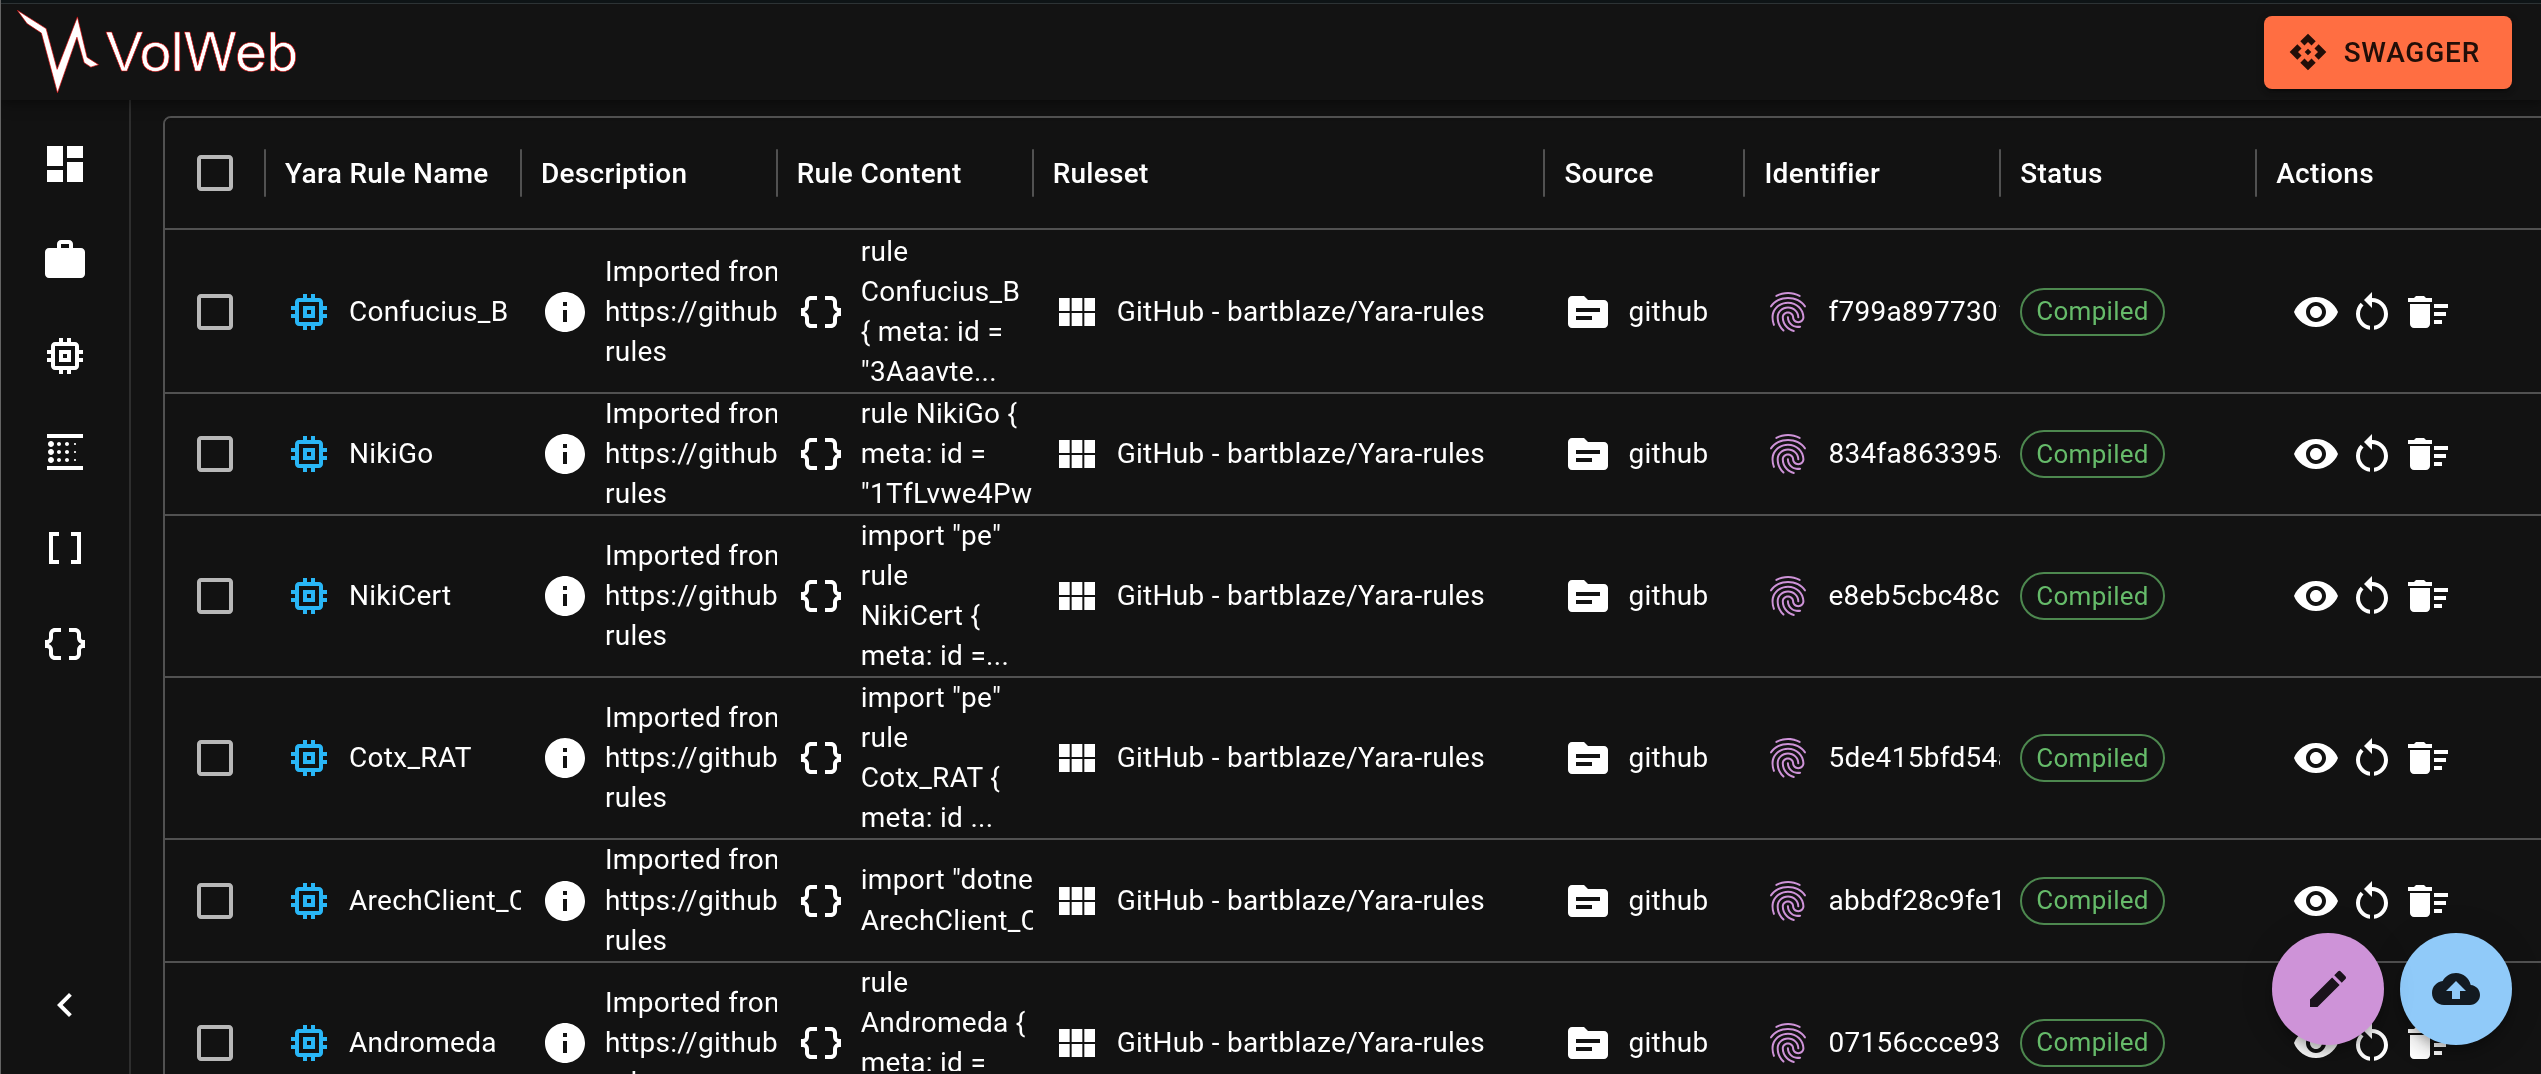
\includegraphics[width=1\linewidth]{images/volweb-esteso/volweb-rulelist.png}
\end{figure}

\subsubsection{Import e Creazione di Regole}

Il sistema di acquisizione delle regole supporta tre modalità principali: upload da file system, import da repository GitHub, e creazione manuale tramite editor integrato.

L'upload da file system implementa un'interfaccia che accetta la selezione di singoli file .yar. Il dialog consente la selezione della modalità di import (regola standalone, ruleset esistente, nuovo ruleset). Durante l'upload, una progress bar mostra l'avanzamento per file, con possibilità di cancellare upload in corso.

L'integrazione GitHub permette import diretto da repository pubbliche, eliminando il download manuale. Il sistema mantiene una lista curata di repository popolari (Yara-Rules, reversinglabs-yara, Neo23x0/signature-base) con accesso one-click. Per repository custom, l'utente può inserire l'URL e il sistema enumera automaticamente tutti i file .yar disponibili. Il sistema mantiene il riferimento alla fonte originale per facilitare aggiornamenti futuri.

L'editor integrato per creazione di regole custom fornisce un ambiente di sviluppo completo. Il componente, basato su Monaco Editor (lo stesso engine di VS Code), offre syntax highlighting specifico per YARA con colorazione differenziata per keywords, strings, e commenti. L'auto-completion suggerisce keywords YARA, nomi di variabili definite, e funzioni built-in mentre si digita. La validazione real-time sottolinea errori sintattici con squiggly lines rosse e mostra tooltip con descrizioni degli errori on hover.

\begin{figure}[H]
\centering
\begin{minipage}{0.45\textwidth}
\centering
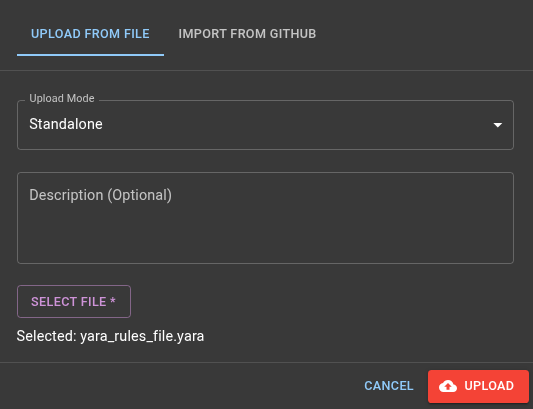
\includegraphics[width=\textwidth,height=6cm]{images/volweb-esteso/volweb-upload-dialog.png}
\end{minipage}
\hspace{0.05\textwidth}
\begin{minipage}{0.45\textwidth}
\centering
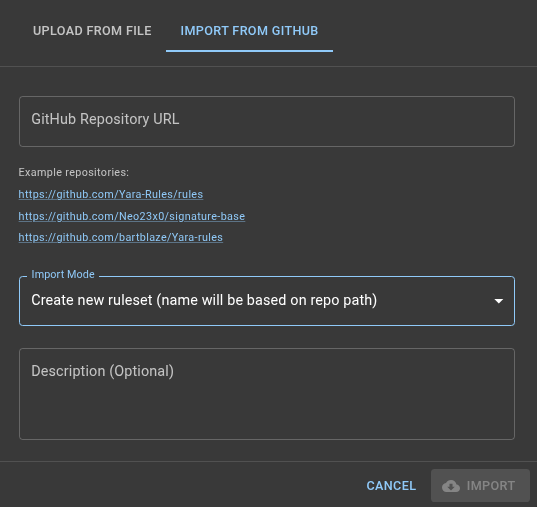
\includegraphics[width=\textwidth,height=6cm]{images/volweb-esteso/volweb-import-dialog.png}
\end{minipage}
\end{figure}

La gestione degli errori durante l'import è stata progettata per essere informativa senza essere overwhelming. Errori di validazione sono raggruppati per tipo e presentati in un formato scannable. Per ogni errore, il sistema mostra la linea esatta dove si verifica il problema, una descrizione human-readable dell'errore, e suggerimenti per la correzione quando possibili. Gli errori non bloccano l'import di altre regole valide, permettendo import parziali con report dettagliato di cosa è stato importato e cosa è fallito.

\subsubsection{Gestione dei RuleSets}

L'implementazione della dashboard dedicata ai ruleset é la stessa della dashboard delle regole, utilizzando Material-UI DataGrid con virtualizzazione delle righe per gestire efficientemente centinaia di ruleset senza degradazione delle performance.

Ogni riga mostra informazioni essenziali ottimizzate per scansione visiva rapida: il nome del ruleset, la sua descrizione, lo stato di compilazione e le azioni rapide disponibili.

Le azioni rapide disponibili per ogni ruleset sono: la visualizzazione dettagliata che reinvia alla vista espansa del ruleset con lista delle regole contenute e stato di ciascuna; la compilazione manuale che permette di ricompilare il ruleset in qualsiasi momento; l'eliminazione, che richiede conferma tramite dialog per prevenire cancellazioni accidentali.

\begin{figure}[H]
\centering
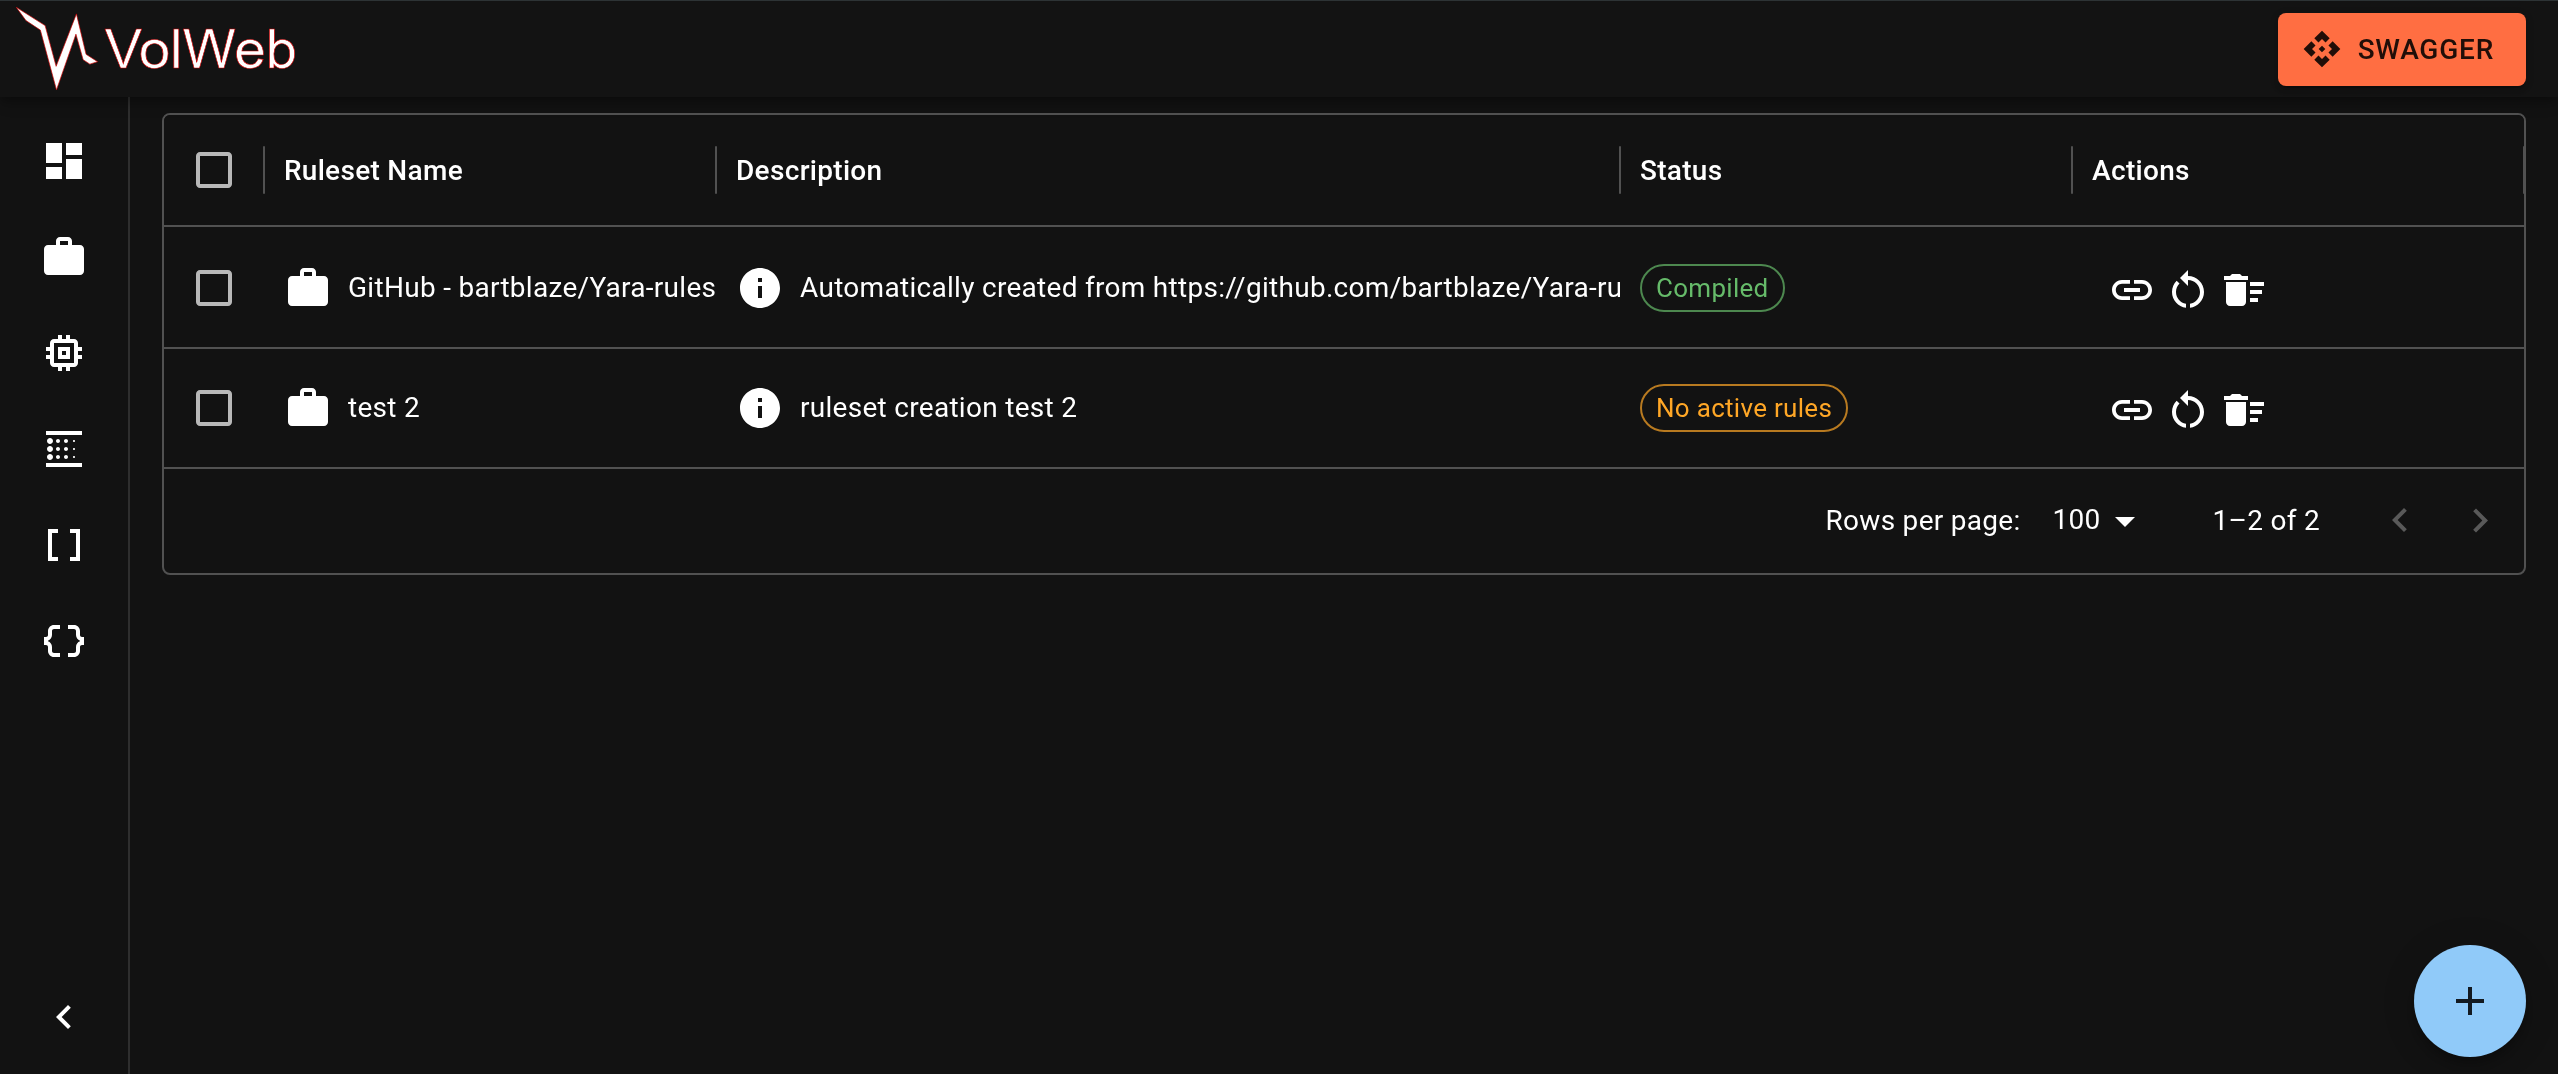
\includegraphics[width=1\linewidth]{images/volweb-esteso/volweb-rulesetlist.png}
\end{figure}

\subsubsection{Configurazione ed Esecuzione delle Scansioni}

L'interfaccia di scansione fornisce controllo sulla selezione delle regole utilizzando un'interfaccia a due pannelli con rulesets sulla sinistra e regole individuali sulla destra. Gli utenti possono selezionare interi rulesets, che automaticamente selezionano tutte le regole attive al loro interno, oppure selezionare regole individuali, o entrambe le modalità. É possibile, infine, selezionare tutti i rulesets e/o tutte le regole attive tramite checkbox dedicate.

Una volta selezionate le regole, l'utente può avviare la scansione, che viene eseguita in background tramite Celery. Al termine della scansione, l'utente viene notificato via WebSocket e può visualizzare i risultati dettagliati.

Alternativamente all'esecuzione di un nuovo scan, l'utente può visualizzare i risultati dell'ultimo scan eseguito sul dump selezionato, se disponibile. Questa funzionalità permette di rivedere rapidamente i risultati senza dover rieseguire la scansione.

\begin{figure}[H]
\centering
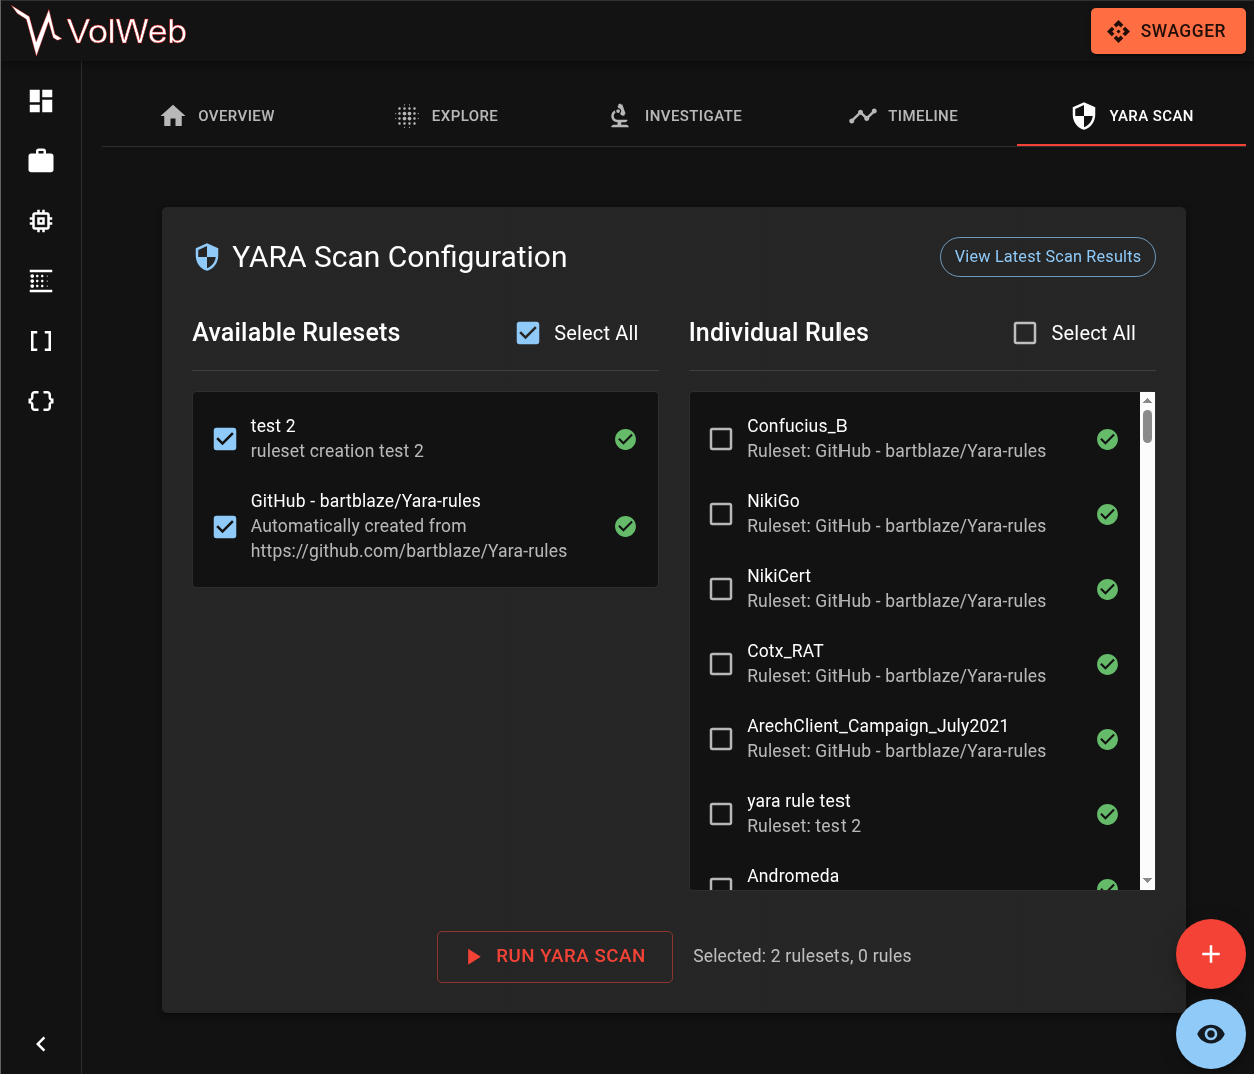
\includegraphics[width=1\linewidth]{images/volweb-esteso/volweb-scanview.png}
\end{figure}

\subsubsection{Visualizzazione e Analisi dei Risultati}

La presentazione dei risultati delle scansioni YARA é organizzata in una vista tabellare con funzionalità di filtering e sorting. 

La tabella, per ogni match, mostra il nome della regola che ha generato il match, il valore che ha causato il match, l'offset esatto nel dump e il componente della regola che é stato attivato.

É possibile eliminare i risultati dello scan corrente, che rimuove tutti i match associati al dump dal database, oppure eseguire un nuovo scan salvando i risultati appena visualizzati.

\begin{figure}[H]
\centering
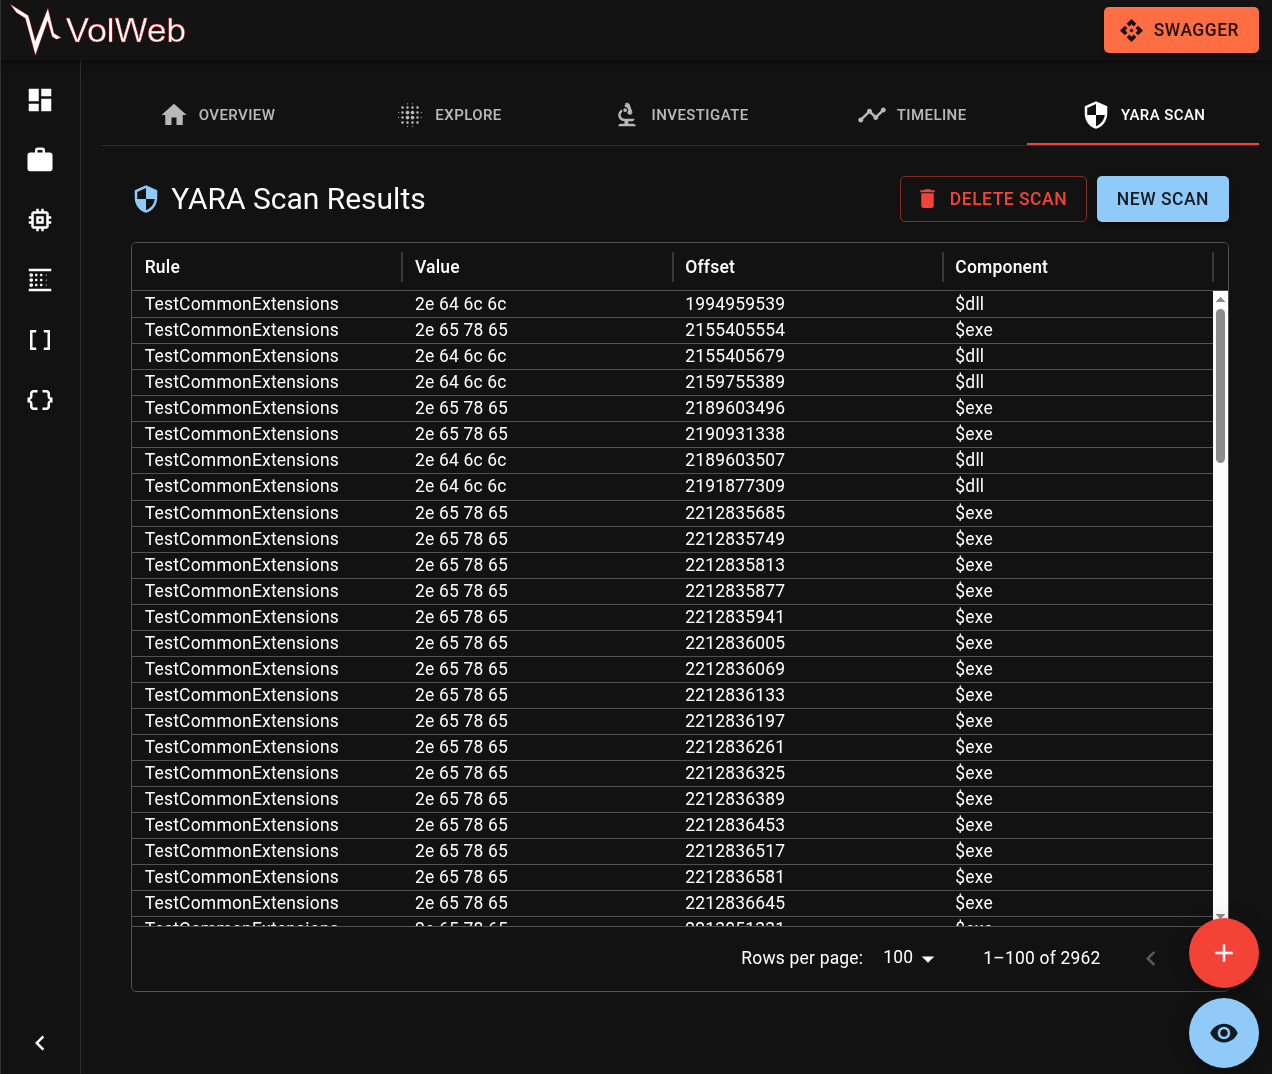
\includegraphics[width=1\linewidth]{images/volweb-esteso/volweb-scanresult.png}
\caption{Visualizzazione stratificata dei risultati YARA con drill-down progressivo dal summary al dettaglio forense}
\end{figure}

\section{Semplificazioni Architetturali}

Parallelamente all'integrazione YARA, sono state implementate semplificazioni architetturali significative basate sull'esperienza operativa di Locked Shields 2025.

\subsection{Rimozione del Sistema di Autenticazione}

L'eliminazione del layer di autenticazione rappresenta una decisione progettuale apparentemente controintuitiva che tuttavia riflette la realtà operativa degli ambienti forensi isolati. Durante Locked Shields 2025, ogni blue team operava in un ambiente di rete completamente segregato dove il controllo degli accessi era demandato all'infrastruttura di rete piuttosto che all'applicazione.

L'analisi dell'utilizzo durante l'esercitazione ha rivelato pattern interessanti. I team tipicamente deployavano VolWeb su una VM isolata accessibile solo dalla rete del team. L'accesso alla rete era già protetto da VPN con autenticazione multi-fattore. All'interno del team, tutti i membri necessitavano dello stesso livello di accesso. Il tempo speso per gestire account utente e password reset durante l'esercitazione rappresentava overhead non produttivo.

Ancora più critico, il sistema di autenticazione rappresentava un vettore di attacco sfruttabile. Durante le simulazioni, i red team targetizzavano specificatamente i sistemi di autenticazione delle applicazioni web.

L'architettura risultante assume che VolWeb venga deployato in ambienti trusted dove la sicurezza perimetrale è già garantita. Questo modello si allinea con il principio di defense in depth, dove la sicurezza non dipende da un singolo controllo ma da layer multipli. Per deployment che richiedono autenticazione, il sistema può essere protetto attraverso reverse proxy (nginx, Apache) con autenticazione integrata, VPN con controlli di accesso basati su certificati, o network segmentation con firewall rules.

\subsection{Eliminazione del Supporto Cloud Storage}

La rimozione del supporto per storage cloud deriva da considerazioni pratiche e di sicurezza emerse durante operazioni reali. L'analisi post-Locked Shields ha rivelato che zero team su 40 hanno utilizzato il cloud storage durante l'esercitazione, nonostante fosse disponibile e configurato.

Le ragioni per il non-utilizzo erano molteplici. Dal punto di vista della sicurezza, i dump di memoria contengono inevitabilmente dati estremamente sensibili. L'upload automatico di tali dati su infrastrutture cloud viola multiple normative di compliance, GDPR per dati personali EU, HIPAA per informazioni sanitarie, PCI-DSS per dati di pagamento, e classificazioni governative per informazioni sensibili.

Dal punto di vista operativo, la dipendenza da servizi cloud introduceva failure points inaccettabili. Durante Locked Shields, i servizi cloud simulati erano tra i primi target degli attacchi red team. In uno scenario reale di incident response, questi problemi sarebbero ancora più critici quando l'infrastruttura aziendale è sotto attacco.

Le considerazioni di performance hanno ulteriormente supportato la decisione. L'upload di dump da 20-64 GB su connessioni internet standard richiedeva ore. Il download per analisi introduceva latenza significativa. I costi di storage e bandwidth per dump multipli diventavano rapidamente proibitivi. La sincronizzazione tra storage locale e cloud aggiungeva complessità senza valore evidente.

L'implementazione della rimozione ha richiesto un refactoring significativo ma ha prodotto un'architettura più semplice e robusta. 

Le espansioni presentate in questo capitolo trasformano VolWeb da una piattaforma di visualizzazione a uno strumento completo per l'analisi forense avanzata. L'integrazione di YARA colma il gap più critico identificato durante Locked Shields 2025, fornendo capacità di pattern matching e threat hunting precedentemente assenti. Le semplificazioni architetturali garantiscono che la piattaforma rimanga accessibile e resiliente anche nei contesti operativi più impegnativi, rimuovendo complessità non necessaria e potenziali punti di failure.

L'implementazione dettagliata, comprensiva di tutto il codice sorgente, è disponibile nel repository GitHub del progetto, come documentato nell'Appendice A.

Il capitolo successivo discuterà i test di validazione eseguiti per garantire che le nuove funzionalità soddisfino i requisiti definiti, seguiti da una valutazione complessiva dell'impatto delle espansioni sulla piattaforma VolWeb.